\documentclass[10pt,article]{article}
\newcommand{\myMargin}{0.2in}
\usepackage[a4paper, margin=\myMargin]{geometry}
\usepackage{graphicx}
\usepackage{booktabs}
\usepackage{url}
\usepackage{enumitem}
\usepackage{palatino}
\usepackage{tabularx}
\usepackage{multicol}
\usepackage{xcolor}
\usepackage{enumitem}
\usepackage[hidelinks]{hyperref}
\fontfamily{SansSerif}
\usepackage{multirow}
% \usepackage{fontspec}
\usepackage{fontawesome}
% \usepackage[T1]{fontenc}

\selectfont

\usepackage[T1]{fontenc}
\usepackage
%[ansinew]
[utf8]
{inputenc}

\usepackage{color}
% \definecolor{myblue}{gray}{0.82}
\definecolor{myblue}{HTML}{96bfeb}
\definecolor{myred}{HTML}{961212}
\definecolor{nptel}{HTML}{c71254}
\textheight=10.75in
\raggedbottom

\setlength{\tabcolsep}{0in}
\newcommand{\isep}{-2 pt}
\newcommand{\lsep}{-0.5cm}
\newcommand{\psep}{-0.6cm}
\renewcommand{\labelitemii}{$\circ$}

\pagestyle{empty}
%-----------------------------------------------------------
%Custom commands
\newcommand{\resitem}[1]{\item #1 \vspace{-2pt}}
% \newcommand{\resheading}[1]{{\small \colorbox{myblue} { \begin{minipage}{0.99\textwidth}\centering{\textbf{#1 \vphantom{p\^{E}}}}\end{minipage}}}}
% \newcommand{\ressubheading}[3]{
% \begin{tabular*}{6.62in}{l @{\extracolsep{\fill}} r}
% 	\textsc{{\textbf{#1}}} & \rightline\textsc{\textit{[#2]}} \\
% \end{tabular*}\vspace{-8pt}}

\newcommand{\resheading}[1]{{\small \colorbox{myblue} { \begin{minipage}{\dimexpr\linewidth-2\fboxsep}\centering{\textbf{#1 \vphantom{p\^{E}}}}\end{minipage}}}}

\newcommand{\ressubheading}[3]{
\begin{tabular*}{\linewidth}{@{}l @{\extracolsep{\fill}} r@{}}
    \textsc{\textbf{#1}} & \textsc{\textit{[#2]}} \\
\end{tabular*}\vspace{-8pt}}

% New command for font size
\newcommand{\myfont}[2]{\fontsize{#1}{#1}\selectfont #2}

% New command for Subheading font size
\newcommand{\subheadingfont}[1]{\myfont{11pt}{#1}}

% New command for Project Topic name 
\newcommand{\projecttopic}[1]{\myfont{11pt}{\textbf{#1}}}

% New command for Project Description
\definecolor{projDescColor}{HTML}{1923A8}
\newcommand{\projectdesc}[1]{\myfont{10pt}{\textcolor{projDescColor}{\textit{#1}}}}

% New command for Link
\newcommand{\mylink}[1]{\href{#1}{
\includegraphics[scale=0.03]{download.png}}}

% New command for Calendar
\newcommand{\mycal}[1]{
\includegraphics[scale=0.018]{calendar.png} \myfont{10}{#1}}

% New command for Location
\newcommand{\myloc}[1]{
\includegraphics[scale=0.7]{loc.png} \myfont{10}{#1}}

%%%%%%%%%%%%%%%%%%%%%%%%%%%%%%%%%%%%%%%%%%%%%%%%%%%%%%%%%%%%%%%%%%%%%%%%%%%%%%%%%%%%%%%%%%%%%%%%%%%%%%%%%%

\begin{document}
\begin{table}
    \begin{minipage}{0\linewidth}
        \centering
        
\includegraphics[height =1in]{Logo.png}
    \end{minipage}
    \begin{minipage}{0.9\linewidth}
        %\centering
        \setlength{\tabcolsep}{70pt}
        \def\arraystretch{1.1}
        \begin{tabular}{l l r}
            \textbf{\Large{Snehadeep Gayen $\vert$ CS21B078}} &
            \multirow{3}{*}{     {\href{https://github.com/Snehadeep-Gayen}{
\includegraphics[scale=0.05]{github.png}} \ 
 \href{https://www.linkedin.com/in/snehadeep-gayen/}{
\includegraphics[scale=0.05]{linkedin.png}} \ \href{https://codeforces.com/profile/Snehadeep}{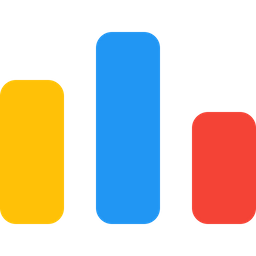
\includegraphics[scale=0.06]{cf.png} \ } 
            }}
            % &  {\href{https://github.com/Snehadeep-Gayen}{
\includegraphics[scale=0.03]{github.png}} \  Snehadeep-Gayen} 
            \\
            \textbf{B. Tech Computer Science and Engineering} 
            \\
            {Indian Institute of Technology, Madras} 
            % &    {\href{https://codeforces.com/profile/Snehadeep}{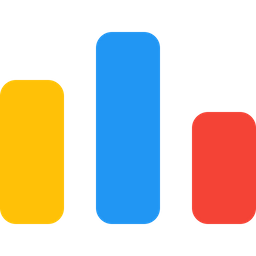
\includegraphics[scale=0.04]{cf.png}} \ Snehadeep} 
            \\
        \end{tabular}
    \end{minipage}\hfill
\end{table}

%%%%%%%%%%%%%%%%%%%%%%%%%%%%%%%%%%%%%%%%%%%%%%%%%%%%%%%%%%%%%%%%%%%%%%%%%%%%%%%%%%%%%%%%%%%%%%%%%%%%%%%%%%

%%%%%%%%%%%%%%%%%%%%%%%%%%%%%%%%%%%%%%%%%%%%%%%%%%%%%%%%%%%%%%%%%%%%%%%%%%%%%%%%%%%%%%%%%%%%%%%%%%%%%%%%%%

\begin{multicols*}{2}


%%%%%%%%%%%%%%%%%%%%%%%%%%%%%%%%%%%%%%%%%%%%%%%%%%%%%%%%%%%%%%%%%%%%%%%%%%%%%%%%%%%%%%%%%%%%%%%%%%%%%%%%%%

\noindent
\resheading{\subheadingfont{EDUCATION}} \\

\noindent
\projecttopic{B. Tech CSE \big \vert \hspace{3pt} CGPA 9.90} \hfill \mycal{Jul '21 - Present} \\
\projectdesc{Indian Institute of Technology Madras}  \hfill \myloc{Chennai, TN}\\

\noindent
\projecttopic{HSC Class 12$^{\mathbf{th}}$ \big \vert \hspace{3pt} 98.17\%} \hfill \mycal{Apr '20 - Apr '21} \\
\projectdesc{Pace Junior Science College}  \hfill \myloc{Mumbai, MH}\\

\noindent
\projecttopic{ICSE Class 10$^{\mathbf{th}}$ \big \vert \hspace{3pt} 98.80\%} \hfill \mycal{Apr '18 - Apr '19} \\
\projectdesc{Lilavatibai Podar High School} \hfill \myloc{Mumbai, MH}\\

%%%%%%%%%%%%%%%%%%%%%%%%%%%%%%%%%%%%%%%%%%%%%%%%%%%%%%%%%%%%%%%%%%%%%%%%%%%%%%%%%%%%%%%%%%%%%%%%%%%%%%%%%%
\noindent
\resheading{\subheadingfont{EXPERIENCE}} \\ [0.1cm]

\noindent
\hrulefill \\ [-0.5cm]
\projecttopic{Team Avishkar Hyperloop, C\textcolor{red}{FI}} \hfill \mycal{Oct '22 - Present} 
\begin{itemize}[leftmargin=\myMargin]
    \item Part of Code Development Team of the \textbf{Main Control Unit} and \textbf{Navigation Unit} of our Pod. 
    \item Used \textbf{RTOS, threading} and communication protocols like MQTT, CAN, etc. to collect and store data from over 20 sensors at \textbf{low latency}, \textbf{handling faults} appropriately.
    % \item Used communication protocols like MQTT, CAN, etc to collect data and send data to the base station/on-Pod Storage.
    \item Participated in the prestigious \textbf{European Hyperloop Week - Scotland 2023}, 
    among over 25 teams globally to represent the country.
\end{itemize}
\vspace{3pt}
\noindent
\hrulefill \\ [-0.5cm]
\projecttopic{Tutor \& Contributor, \textcolor{nptel}{NPTEL}} \hfill \mycal{March '23 - Present}
\begin{itemize}[leftmargin=\myMargin]
    \item Created \textbf{YouTube tutorials} for previous years' GATE CS questions
    \item These tutorials aim to support applicants who may have limited access to resources
\end{itemize}

%%%%%%%%%%%%%%%%%%%%%%%%%%%%%%%%%%%%%%%%%%%%%%%%%%%%%%%%%%%%%%%%%%%%%%%%%%%%%%%%%%%%%%%%%%%%%%%%%%%%%%%%%%

\noindent
\resheading{\subheadingfont{CODING ACHIEVEMENTS}}
 \begin{itemize}[ leftmargin=\myMargin]
    \setlength \itemsep{-0.1em}
  \item Maximum Rating 1678 \textcolor{blue}{(Expert)} on Codeforces
%   \item Maximum Rating 1653 \textcolor{blue}{(3 
\includegraphics[scale=0.03]{bluestar.png})} on CodeChef
  \item \textbf{ICPC 2022} - \textbf{AIR 151} and \textbf{Institute Rank 7} in Kanpur-Mathura Qualifier Round
\item \textbf{AIR 3} in Shaastra CP Potpourri (Mixed-bag coding contest) \\ \small {\textit{[Shaastra is Asia's largest student-run Techfest]}} 
    \item \normalsize{ \textbf{Global Rank 9} in CodeChef Starters 96} 
    \item \normalsize{ \textbf{Global Rank 231} in Codeforces Round 881} 
    \item \normalsize{ \textbf{Global Rank 373} in Google Farewell Round B} 
    \item  \normalsize {1st place in Inter-School Java Competition in Mumbai}
  \end{itemize}

%%%%%%%%%%%%%%%%%%%%%%%%%%%%%%%%%%%%%%%%%%%%%%%%%%%%%%%%%%%%%%%%%%%%%%%%%%%%%%%%%%%%%%%%%%%%%%%%%%%%%%%%%%

 
\noindent
\resheading{\subheadingfont{SOFTWARE SKILLS}}
 \begin{itemize}[leftmargin=\myMargin]
    \setlength \itemsep{-0.1em}
  \item \textbf{Languages}: C++, C, HDL (Verilog), Python, Java, HTML, CSS, x86, RISC and 8085 ASM, R
  \item \textbf{Tools}: TI CCS, Git, \textbf{\LaTeX}, AutoCAD, GDB
\item \textbf{Libraries}: TI RTOS, NumPy, PyLops, Matplotlib
  \end{itemize}
  

%%%%%%%%%%%%%%%%%%%%%%%%%%%%%%%%%%%%%%%%%%%%%%%%%%%%%%%%%%%%%%%%%%%%%%%%%%%%%%%%%%%%%%%%%%%%%%%%%%%%%%%%%%

\noindent
\resheading{\subheadingfont{EXTRACURRICULAR ACTIVITIES}}
\begin{itemize}[leftmargin=\myMargin]
    \setlength \itemsep{-0.08em}
\item \textbf{Sports:} Taekwondo Red Dan II Belt, Awarded Best \\ Athlete U14 at School,  School Sports Captain for 2019-20  \\
    Awarded 13 medals in various Track \& Field events in High School, NSO Athlete at IITM
\item Mentored freshmen, personally and academically, \\ under \textbf{Saathi, IIT Madras}
\item Avid book reader and Tabla player
\end{itemize}

%%%%%%%%%%%%%%%%%%%%%%%%%%%%%%%%%%%%%%%%%%%%%%%%%%%%%%%%%%%%%%%%%%%%%%%%%%%%%%%%%%%%%%%%%%%%%%%%%%%%%%%%%%
  

\columnbreak

%%%%%%%%%%%%%%%%%%%%%%%%%%%%%%%%%%%%%%%%%%%%%%%%%%%%%%%%%%%%%%%%%%%%%%%%%%%%%%%%%%%%%%%%%%%%%%%%%%%%%%%%%%

\noindent
\resheading{\subheadingfont{SCHOLASTIC ACHIEVEMENTS}}
\begin{itemize}[leftmargin=\myMargin]
\setlength \itemsep{-0.1em}
\item Secured \textbf{AIR 5} in JEE Mains out of 1 million students  %\hfill {[20XX]}%
\item Secured \textbf{AIR 161} in JEE Advanced \hfill
\item Secured \textbf{AIR 10} in Indian Statistical Institute Exam
\item Secured \textbf{AIR 21} in INChO and attended Orientation Camp for International Chemistry Olympiad
\item Awarded KVPY Fellowship '21 with \textbf{AIR 338}
\item Winner of Mimamsa '22 at IISER Pune \\ 4$^{th}$ place in Chemenigma '22 at IISC Bangalore \& \\ Won Silver Medal in Homi Bhabha Science Competition \\ (conducted in Maharashtra)
\end{itemize} 

%%%%%%%%%%%%%%%%%%%%%%%%%%%%%%%%%%%%%%%%%%%%%%%%%%%%%%%%%%%%%%%%%%%%%%%%%%%%%%%%%%%%%%%%%%%%%%%%%%%%%%%%%%
    
\noindent
\resheading{\subheadingfont{PROJECTS} }\\[0.1cm]

\noindent
\hrulefill \\ [-0.5cm]
\projecttopic{WiFi Tomography} \textit{\myfont{9pt}{(Ongoing)}} \hfill \textcolor{projDescColor}{\textit{Python}}  \\[0.1cm]
\projectdesc{Project Under Prof. Ayon Chakraborty} \hfill \mycal{May'23 - Present} 
\begin{itemize}[leftmargin=\myMargin]
    \item WiFi tomography is a low-cost and easily implementable method to image the environment using WiFi signals.
    \item Working on computational optimisation of Tomographic Reconstruction to make it suitable for outdoor
        and indoor drone application 
\end{itemize} 
\vspace{5pt}

\noindent
\hrulefill \\ [-0.5cm]
\projecttopic{CPU Design} \mylink{https://github.com/Snehadeep-Gayen/Computer-Organisation-and-Architecture-Lab} 
\mylink{https://github.com/Snehadeep-Gayen/Simple_CPU_Design} 
\hfill    \textcolor{projDescColor}{\textit{Verilog}}  \\[0.1cm]
\projectdesc{CS2610 Course Project - Prof. C. Chandra Sekhar} \hfill \mycal{Jan-May '23} \\
\projectdesc{CS2310 Course Project - Prof. Ayon Chakraborty} \hfill \mycal{Jul-Nov '22}
\noindent
\begin{itemize}[leftmargin=\myMargin]
    \item Implemented a CPU with register file and ALU with instructions to perform Arithmetic 
    and Logical operations on both 8-bit integers and  12-bit floating-point numbers
    \item Built a combinational 8-bit CPU from gate level
\end{itemize}
\vspace{5pt}

\noindent
\hrulefill \\ [-0.5cm]
\projecttopic{Reading Project and Presentation} \mylink{https://docs.google.com/presentation/d/11JGNKZnVHHQ-aGJLIgkdXcnK5qy_xisO/edit?usp=sharing&ouid=111499804735475673896&rtpof=true&sd=true} \\ [0.1cm]
\projectdesc{CS6122 Course Project - Prof. B. V. R. Rao} \hfill \mycal{Jan-May '23} 
\begin{itemize}[leftmargin=\myMargin]
    \item Presented the paper on \href{https://doi.org/10.1007/s00453-012-9643-5}{\textit{``Smoothed Analysis of Partitioning Algorithms for Euclidean Functionals"} 
    by \textit{Bläser, M., Manthey, B. \& Rao, B.V.R.}} and discussed its applications to problems
\end{itemize}
\vspace{5pt}

\noindent
\hrulefill \\ [-0.5cm]
\projecttopic{Closeness Centrality Algorithm} \mylink{https://github.com/Snehadeep-Gayen/CENDY-Incremental-CC}
 \hfill \textcolor{projDescColor}{\textit{C++}} \\ [0.1cm]
\projectdesc{Project under Prof. Manikandan Narayanan} \hfill \mycal{May-Jun '23}
\begin{itemize}[leftmargin=\myMargin]
    \item Implemented the CENDY algorithm based on this paper \ \mylink{https://ieeexplore.ieee.org/stamp/stamp.jsp?tp=&arnumber=6729571&isnumber=6729471}
    \item This on-line algorithm updates Average Path Length and Closeness Centrality of all nodes
    in a Dynamic Graph
 \end{itemize}
%%%%%%%%%%%%%%%%%%%%%%%%%%%%%%%%%%%%%%%%%%%%%%%%%%%%%%%%%%%%%%%%%%%%%%%%%%%%%%%%%%%%%%%%%%%%%%%%%%%%%%%%%%



%%%%%%%%%%%%%%%%%%%%%%%%%%%%%%%%%%%%%%%%%%%%%%%%%%%%%%%%%%%%%%%%%%%%%%%%%%%%%%%%%%%%%%%%%%%%%%%%%%%%%%%%%%


\noindent
\resheading{\subheadingfont{COURSES \& LABS}}
 % \textbf{Econometrics \big\vert \   Statistics \big\vert \   Mathematical Methods \big\vert \   Microeconomics \big\vert \   Macroeconomics}\hfill {[ISI-D]}\\[-0.1cm]\\
\begin{multicols}{2} 

\begin{itemize}[ leftmargin=\myMargin]
    \setlength \itemsep{-0.2em}
  % \item {\small Problem Solving using Computers} 
  \item { Basic Electrical Engg} 
  \item { Computer Systems Design} 
  \item {Programming and Data Structures}
  \item { Computer Organisation and Architecture} 
  \item { Design \& Analysis of  \\ Algorithms} 
  \item { Theory of Computation} 
  \item { Probabilistic, Smoothed Analysis of Algorithms (PG)} 
  \item { Object Oriented Programming} 
  \item { Discrete Maths} 
  \item { Basic Graph Theory} 
  \item { Probability, Statistics \& Stochastic Processes} 
  \item { Series and Matrices} 
  \item { Multivariable Calculus} 
  \item { Ordinary Differential Equations (PG)}  
  \item { Principles of Economics} 
  \item { Intro to Game Theory}   
  \item { Compiler Design *} 
  \item { Operating System *}
\end{itemize}
\hfill  {* ~ Ongoing}

\end{multicols}

%%%%%%%%%%%%%%%%%%%%%%%%%%%%%%%%%%%%%%%%%%%%%%%%%%%%%%%%%%%%%%%%%%%%%%%%%%%%%%%%%%%%%%%%%%%%%%%%%%%%%%%%%%

\end{multicols*}
\end{document}